%%%%%%%%%%%%%%%%%%%%%%%%%%%%%%%%%%%%%%%%%
% NIWeek 2014 Poster by T. Reveyrand
% www.microwave.fr
% http://www.microwave.fr/LaTeX.html
% ---------------------------------------
%
% Original template created by:
% Brian Amberg (baposter@brian-amberg.de)
%
% This template has been downloaded from:
% http://www.LaTeXTemplates.com
%
% License:
% CC BY-NC-SA 3.0 (http://creativecommons.org/licenses/by-nc-sa/3.0/)
%
%%%%%%%%%%%%%%%%%%%%%%%%%%%%%%%%%%%%%%%%%

%----------------------------------------------------------------------------------------
%   PACKAGES AND OTHER DOCUMENT CONFIGURATIONS
%----------------------------------------------------------------------------------------

\documentclass[a0paper,portrait]{baposter}

\usepackage[font=small,labelfont=bf]{caption} % Required for specifying captions to tables and figures
\usepackage{booktabs} % Horizontal rules in tables
\usepackage{relsize} % Used for making text smaller in some places

\usepackage{amsmath,amsfonts,amssymb,amsthm} % Math packages
\usepackage{eqparbox}
\usepackage{textcomp}
\usepackage{caption}
\usepackage{subcaption}
\usepackage{graphicx}
\usepackage{listings}
\usepackage{mathtools}
\usepackage{multirow}
\usepackage[percent]{overpic}
%\usepackage{hyperref}

%\usepackage{pgf}

\usepackage[utf8]{inputenc}
\usepackage{tikz}
\usetikzlibrary{calc}
\usetikzlibrary{shapes,arrows}
\usetikzlibrary{arrows,automata}
\usetikzlibrary{positioning}
\usetikzlibrary{shapes.callouts}


\usepackage{multicol}
\usepackage{hyperref}
\usepackage[font=small,labelfont=bf]{caption}
\usepackage{makecell}
\usepackage{enumitem}
\usepackage{fontawesome}
\usepackage{xparse}


\newcommand{\tikzmark}[1]{\tikz[overlay,remember picture] \node (#1) {};}
\def\Put(#1,#2)#3{\leavevmode\makebox(0,0){\put(#1,#2){#3}}}

%\tikzset{
%    invisible/.style={opacity=0,text opacity=0},
%    visible on/.style={alt=#1{}{invisible}},
%    alt/.code args={<#1>#2#3}{%
%      \alt<#1>{\pgfkeysalso{#2}}{\pgfkeysalso{#3}} % \pgfkeysalso doesn't change the path
%    },
%}

\NewDocumentCommand{\mycallout}{r<> O{opacity=0.8,text opacity=1} m m}{%
\tikz[remember picture, overlay]\node[align=center, fill=cyan!20, text width=3.5cm,
#2, rounded corners,
draw,rectangle callout,anchor=pointer,callout relative pointer={(230:1cm)}]
at (#3) {#4};
}

\renewcommand\theadalign{bc}
\renewcommand\theadfont{\bfseries}
\renewcommand\theadgape{\Gape[4pt]}
\renewcommand\cellgape{\Gape[4pt]}

%for [[ ]]
\usepackage{stmaryrd}

\setlist[itemize]{leftmargin=*}

\graphicspath{{figures/}} % Directory in which figures are stored

 \definecolor{bordercol}{RGB}{40,40,40} % Border color of content boxes
 \definecolor{headercol1}{RGB}{210,235,250} % Background color for the header in the content boxes (left side)
 \definecolor{headercol2}{RGB}{210,235,250} % Background color for the header in the content boxes (right side)
 \definecolor{headerfontcol}{RGB}{0,0,0} % Text color for the header text in the content boxes
 \definecolor{boxcolor}{RGB}{240,255,255} % Background color for the content in the content boxes

\tikzset{
    state/.style={
           ellipse,
           draw=black, thin,
           minimum height=0.5cm,
           minimum width=0.6cm,
           text centered,
           font=\scriptsize
           },
    horiz/.style={
           % font=\tiny,
           inner sep=3pt,
           font=\bf

           } ,
    point/.style={
           circle,
           minimum width = 5pt,
           fill
           }
}

\begin{document}

\setlength{\fboxsep}{0pt}

\background{ % Set the background to an image (background.pdf)
\begin{tikzpicture}[remember picture,overlay]
\draw (current page.north west)+(-2em,2em) node[anchor=north west]
{\includegraphics[height=1.1\textheight]{background}};
\end{tikzpicture}
}

\begin{poster}{
grid=false,
columns=12, % because reasons
borderColor=bordercol, % Border color of content boxes
headerColorOne=headercol1, % Background color for the header in the content boxes (left side)
headerColorTwo=headercol2, % Background color for the header in the content boxes (right side)
headerFontColor=headerfontcol, % Text color for the header text in the content boxes
boxColorOne=boxcolor, % Background color for the content in the content boxes
headershape=rectangle, % Specify the rounded corner in the content box headers
headerfont=\Large\sf\bf, % Font modifiers for the text in the content box headers
textborder=none,
background=none,
headerborder=none, % Change to closed for a line under the content box headers
boxshade=plain
}
{\includegraphics[width=2.5cm]{figures/PPoPP.pdf}}
%
%----------------------------------------------------------------------------------------
%   TITLE AND AUTHOR NAME
%----------------------------------------------------------------------------------------
%
{\bf \huge{Optimizing GPU Programs By Partial Evaluation} }
%\\  \Large \it Context-free grammars and neural networks for secondary structure} % Poster title
{\vspace{0.6em} \smaller \textbf{Semyon Grigorev} \\  % Author names
\smaller \it {JetBrains Research, Saint Petersburg University, Russia } \\ % Author email addresses
\smaller  {s.v.grigoriev@spbu.ru, Semyon.Grigorev@jetbrains.com}}
{\includegraphics[width=2.5cm]{SPbGU_Logo.png}} % University/lab logo


%----------------------------------------------------------------------------------------
%   INTRODUCTION
%----------------------------------------------------------------------------------------
\begin{posterbox}[name=CFPQ,column=0,row=0, span=4]{Problem Statement}

  Memory traffic is a bottleneck of GPGPU programms.
  There are cases of data analysis when some of kernel parameters are fixed during many kernel runs.
  \begin{itemize}
    \item Patterns in substring matching
    \item HMM in homology search
    \item Query in graph database qurying
  \end{itemize}
  Known parameters are still increase memory traffic. \textbf{Can we automatically opimize procedire with partially known parameters?}
\end{posterbox}

\headerbox {Example}
{name=matrices,column=0,span=6, row=2, below=CFPQ}%,bottomaligned=sol2}
{
\includegraphics[width=0.99\textwidth]{CodeSample1.pdf}
}

\headerbox {Results}{name=results,column=4,row=0, span=4, bottomaligned=CFPQ}{
\begin{itemize}
  \item It is possible to optimize procedures with partially known parameters by using \textbf{partial evaluation}~\cite{Jones:1993:PEA:153676}
  \begin{itemize}
    \item Optimized procedure for substring matching is up to 2 times faster
    \item !!!
  \end{itemize}
  \end{itemize}
}

\headerbox {Future Research}{name=answers,column=8,row=0, span=4, bottomaligned=results}{

  \begin{itemize}
    \item Switch to CUDA C partial evaluator.
    \begin{itemize}
      \item LLVM.mix: partial evaluator for LLVM IR.
    \end{itemize}
    \item Reduce specialization overhead to make it applicable in run-time.
    \item Integrete with shared memory register spilling~\cite{DBLP:journals/corr/abs-1907-02894}.
    \item Evaluate on real-world examples.
    \begin{itemize}
      \item Homology search in bioinformatics.
      \item Graph processing.
      %\item Graph database querying.
    \end{itemize}
  \end{itemize}

}


\headerbox {Partial Evaluation~\cite{Jones:1993:PEA:153676}}
{name=impl,column=6,span=6, row=2, below=results,bottomaligned=matrices}
{
\vspace{-0.4cm}
{\small{$$
%\begin{multline}
   \llbracket \underbrace{handleData}_{handleData} \rrbracket [filterParams, data] =
   \llbracket \underbrace{\overbrace{mix}^{\mathclap{\text{partial evaluator}}} \rrbracket [handleData,filterParams]}_{handleData_{mix}}\rrbracket [data]
%\end{multline}
$$}}
%\vspace{5cm}

\hspace{7cm}$\llbracket mix \rrbracket [handleData,[|2;3|]]$\\

\includegraphics[width=0.99\textwidth]{CodeSample2.pdf}
}




\headerbox{Evaluation: Substring Matching}{name=rdfs,span=9,column=3,row=3,below=matrices}{
%\vspace{0.05cm}
%\begin{table}[h]
%\rowcolors{1}{}{red}
\begin{minipage}[t]{0.3\textwidth}
  \vspace{0pt}
Application: data curving in cyber forensics \\
Subject string: byte array from real hard drive \\
Patterns: !!!!
\end{minipage}
\begin{minipage}[t]{0.35\textwidth}
  \vspace{0pt}
  \begin{overpic}[width=0.9\textwidth]{Substr_1070-crop}
    \put (50,65) {{GTX-1070}}
  \end{overpic}
\end{minipage}
\begin{minipage}[t]{0.35\textwidth}
  \vspace{0pt}
  \begin{overpic}[width=0.9\textwidth]{Substr_T4-crop}
    \put (50,65) {{T4}}
  \end{overpic}
\end{minipage}
}

\headerbox{Implementation}{name=impl,span=3,column=0,row=3,below=matrices}{
We use AnyDSL~\cite{LeiBa} framework for ahead-of-time partial evaluation.
\begin{itemize}
  \item Substring matching: partially evaluated na\"{\i}ve implementation and na\"{\i}ve implementation with different locations of patterns.
  \item 2D convolution: partially evaluated !!!!! from nvidia examples !!!! with unrolled loops by using predefined filter dianetr
  \end{itemize}

}

\setlength{\tabcolsep}{5pt}
\headerbox{Evaluation: 2D Convolution}{name=scaling,span=9,column=3,row=2,below=rdfs}{
\begin{minipage}[t]{0.3\textwidth}
  \vspace{0pt}
Application: data curving in cyber forensics \\
Subject string: byte array from real hard drive \\
Patterns: !!!!
\end{minipage}
\begin{minipage}[t]{0.35\textwidth}
  \vspace{0pt}
  \includegraphics[width=0.9\textwidth]{Conv_1070-crop}
\end{minipage}
\begin{minipage}[t]{0.35\textwidth}
  \vspace{0pt}
  \includegraphics[width=0.9\textwidth]{Conv_T4-crop}
\end{minipage}
}

\headerbox{Hardware}{name=hardware,span=3,column=0,row=2,below=impl,bottomaligned=scaling}{

\begin{itemize}
  \item GTX-1070:
  \item T4:
  \end{itemize}

}

\headerbox {\smaller{Contact Us}}{name=contact,column=0,span=5,below=scaling}{
\scriptsize
\begin{minipage}[t]{0.65\textwidth}
  \vspace{-3cm}
Our team:
\begin{itemize}
  \item Semyon Grigorev: \href{mailto:s.v.grigoriev@spbu.ru}{s.v.grigoriev@spbu.ru}
  \item Nikita Mishin: \href{mailto:mishinnikitam@gmail.com}{mishinnikitam@gmail.com}
  \item Iaroslav Sokolov: \href{mailto:sokolov.yas@gmail.com}{sokolov.yas@gmail.com}
  %\item Egor Spirin: \href{mailto:egor@spirin.tech}{egor@spirin.tech}
  %\item Egor Nemchinov: \href{mailto:nemchegor@gmail.com}{nemchegor@gmail.com}
\end{itemize}


\end{minipage}
~
\begin{minipage}[t]{3cm}

\includegraphics[width=3cm]{qr-research-jetbra.pdf}
\end{minipage}
%\begin{itemize}
%  \item Vladimir Kutuev: \href{mailto:vladimir.kutuev@gmail.com}{vladimir.kutuev@gmail.com}
%  \item Sergey Gorbatyuk: \href{mailto:sergeygorbatyuk171@gmail.com}{sergeygorbatyuk171@gmail.com}
%\end{itemize}
\vspace{1cm}
{\normalsize
Both dataset and implementations are available on GitHub:\\
\url{https://github.com/SokolovYaroslav/CFPQ-on-GPGPU}
}



}

\headerbox{\smaller{References}}{name=references,column=5,span=7,below=scaling}{

    \scriptsize % Reduce the font size in this block
    \renewcommand{\section}[2]{\vskip 0.05em} % Get rid of the default "References" section title
    \nocite{*} % Insert publications even if they are not cited in the poster
    \bibliographystyle{unsrt}
    \bibliographystyle{IEEEtran}
    \bibliography{biblio} % Use biblio.bib as the bibliography file
}

\headerbox {\smaller{Acknowledgments}}{name=ack,column=5,span=7,below=references,bottomaligned=contact}{
\small
The research is supported by the JetBrains Research grant and the~Russian Science Foundation grant 18-11-00100
}


\end{poster}


\end{document}
